% (C) 2016 Jean Nassar. Some Rights Reserved
% Except where otherwise noted, this work is licensed under the Creative Commons Attribution-ShareAlike License, version 4
% Appendices
\appendix
\chapter{System Details}
\section{AR.Drone}
The drone used in this research is the Parrot AR.Drone 2.0 Elite Edition.
It was released by Parrot SA in 2012.
An image is shown in \fref{fig:ardrone}.

\begin{figure}[h]
  \centering
  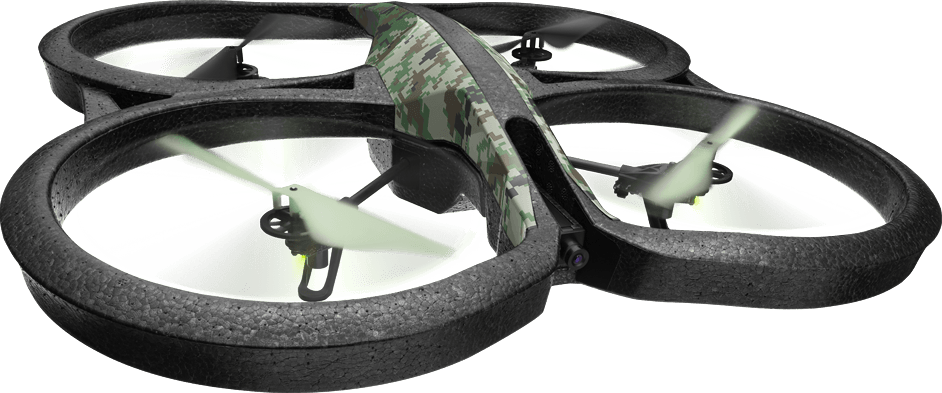
\includegraphics[width=0.5\textwidth]{ardrone}
  \caption[AR.Drone]{AR.Drone 2.0 Elite Edition}
  \label{fig:ardrone}
\end{figure}

Technical specifications are shown in \tref{tab:ardrone_specs}.

\begin{table}[h]
  \centering
  \caption[AR.Drone specifications]{The specifications of the AR.Drone.}
  \begin{tabular}{ll}
    \toprule
    Item & Value \\
    \midrule
    Resolution & 720\,p\\
    Framerate & 30\,fps\\
    Field of view & 92°\\
    Connection & Wi-Fi\\
    Gyroscope  &	3 axles, accuracy of 2,000°/second\\
    Accelerometer  &	3 axles, accuracy of +/- 50\,mg\\
    Magnetometer  &	3 axles, accuracy of 6°\\
    Pressure sensor  & Accuracy of +/- 10\,Pa\\
    Altitude ultrasound sensor  & Measures altitude\\
    Brushless motor power & 14.5\,W\\
    Brushless motor speed & 28,500\,rpm\\
    Weight with indoor frame & 420\,g\\
    \bottomrule
  \end{tabular}
  \label{tab:ardrone_specs}
\end{table}

\section{Motion capture system}
The motion capture system is a set of ten Prime 17W cameras from Optitrack.
One is shown in \fref{fig:mocap_camera}, and technical specifications are in \tref{tab:mocap_specs}.

\begin{figure}[h]
  \centering
  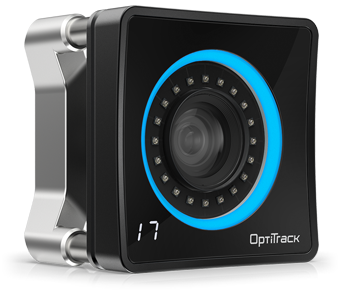
\includegraphics[width=0.5\textwidth]{mocap_camera}
  \caption[Motion capture camera]{The Prime 17W motion capture camera.}
  \label{fig:mocap_camera}
\end{figure}

\begin{table}[h]
  \centering
  \caption[Webcam specifications]{The specifications of the iBuffalo BSW20KM11 webcam.}
  \begin{tabular}{ll}
    \toprule
    Item & Value \\
    \midrule
    Resolution & $1644\times1088$\,pixels\\
    Framerate & 30--360\,fps\\
    Latency & 2.8\,ms\\
    Horizontal field of view & 70°\\
    Vertical field of view & 49°\\
    Filter & 850\,nm band-pass\\
    \bottomrule
  \end{tabular}
  \label{tab:mocap_specs}
\end{table}

\section{Motion capture computer}
The motion capture computer is a Clevo W255HS, running Windows 7 Enterprise.
Its specifications are in \tref{tab:clevo_mocap}.

\begin{table}[h]
  \centering
  \caption[Motion capture computer specifications]{The specifications of the Clevo W255HS computer used to interface with the motion capture system.}
  \begin{tabular}{ll}
    \toprule
    Item & Value \\
    \midrule
    Processor & Intel Core i7-2860QM CPU @ 2.50\,GHz\\
    GPU & nVidia GEFORCE GT 630M, 1\,GB\\
    RAM & 8\,GB\\
    Bits & 64 \\
    \bottomrule
  \end{tabular}
  \label{tab:clevo_mocap}
\end{table}

\section{Operating station}
  The operating station is a Clevo W370ET running Kubuntu 16.10.
  Its specifications are in \tref{tab:clevo_opstn}.

  \begin{table}[h]
    \centering
    \caption[Operating station computer specifications]{The specifications of the Clevo W370ET computer used as the operating station.}
    \begin{tabular}{ll}
      \toprule
      Item & Value \\
      \midrule
      Processor & Intel Core i7-3630QM CPU @ 2.40\,GHz\\
      GPU & nVidia GEFORCE GT 660M, 2\,GB\\
      RAM & 8\,GB\\
      Bits & 64 \\
      \bottomrule
    \end{tabular}
    \label{tab:clevo_opstn}
  \end{table}

\section{Docker environment}
  For the \gls{docker} container that \gls{spirit} runs in, the base is from \texttt{\detokenize{ros:kinetic-robot}}.

  The following ROS packages are installed:

  \begin{itemize}
    \item \textsf{\detokenize{ardrone-autonomy}}
    \item \textsf{\detokenize{image-proc}}
    \item \textsf{\detokenize{mocap_optitrack}}
    \item \textsf{\detokenize{usb_cam}}
  \end{itemize}

  \gls{python} 2.7.13 is installed, with the following dependencies needed for running \gls{spirit}.

  \begin{itemize}
    \item \textsf{\detokenize{catkin_pkg}}
    \item \textsf{\detokenize{defusedxml}}
    \item \textsf{\detokenize{lxml}}
    \item \textsf{\detokenize{numpy}}
    \item \textsf{\detokenize{pygame}}
    \item \textsf{\detokenize{pyyaml}}
    \item \textsf{\detokenize{rospkg}}
    \item \textsf{\detokenize{tqdm}}
  \end{itemize}


\section{External interfaces}
The controller used was an off-the-shelf PlayStation3 controller.

The webcam used to record the experiments was a BSW20KM11 by iBuffalo.
It is shown in \fref{fig:webcam}, and its technical specifications are in \tref{tab:webcam_specs}.

\begin{figure}[h]
  \centering
  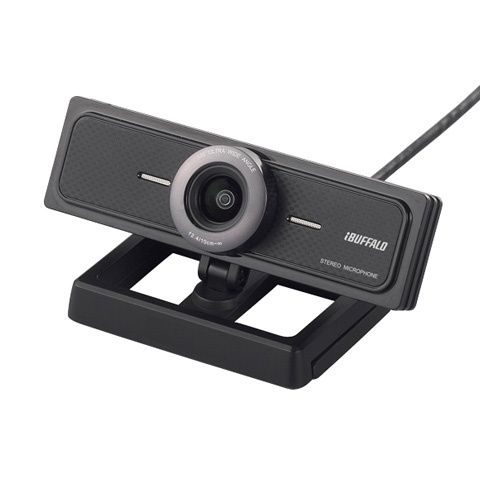
\includegraphics[width=0.5\textwidth]{webcam}
  \caption[Webcam]{The BSW20KM11 webcam.}
  \label{fig:webcam}
\end{figure}

\begin{table}[h]
  \centering
  \caption[Webcam specifications]{The specifications of the iBuffalo BSW20KM11 webcam.}
  \begin{tabular}{ll}
    \toprule
    Item & Value \\
    \midrule
    Resolution & 1080\,p\\
    Framerate & 30\,fps\\
    Field of view & 120°\\
    Microphone & Stereo \\
    \bottomrule
  \end{tabular}
  \label{tab:webcam_specs}
\end{table}


\chapter{Tabulated data}
The means and standard deviations of various measures are shown below.

\section*{Numerical data}
\begin{table}[h]
  \centering
  \caption[Numerical data \sym{mean} and \sym{std}]{The means and standard deviations of the numerical data.}
  \begin{tabular}{lllll}
    \toprule
    & \multicolumn{2}{c}{Onboard} & \multicolumn{2}{c}{\gls{spirit}} \\
    Component & $\sym{mean}$ & $\sym{std}$ & $\sym{mean}$ & $\sym{std}$ \\
    \midrule
    Distance (m) & 0.666 & 0.284 & 0.401 & 0.238\\
    \sym{posx}-position (m) & 0.038 & 0.43 & 0.136 & 0.171\\
    \sym{posy}-position (m) & $-0.474$ & 0.447 & $-0.067$ & 0.366\\
    \gls{rmse}$_{\sym{posx}}$ (m) & 0.338 & 0.191 & 0.192 & 0.122\\
    \gls{rmse}$_{\sym{posy}}$ (m) & 0.52& 0.293 & 0.338 & 0.222\\
    Duration (s) & 39.041 & 18.817 & 44.081 & 15.02\\
    Path length (m) & 10.859 & 2.703 & 11.913 & 2.683\\
    Movement in $\sym{posx}$ (m) & 2.848 & 1.055 & 2.948 & 1.009\\
    Movement in $\sym{posy}$ (m) & 1.051 & 0.579 & 1.273 & 0.698\\
    \bottomrule
  \end{tabular}
  \label{tab:mean_sd}
\end{table}

\begin{table}[h]
  \centering
  \caption[Numerical data $\Delta$\sym{mean} and \sym{effect}]{Difference of means and effect size of the numerical data. The 95\% \gls{ci} is in parentheses.}
  \begin{tabular}{lll}
    \toprule
    Component & $\Delta\sym{mean}$ & \sym{effect} \\
    \midrule
    Distance (m) & 0.266 (0.004, 0.486) & 1.053 ($-0.029$, 2.143)\\
    \sym{posx}-position (m) & $-0.096$ ($-0.35$, 0.206) & $-0.323$ ($-1.266$, 0.56)\\
    \sym{posy}-position (m) & $-0.41$ ($-0.749$, $-0.054)$ & $-1.026$ ($-1.937$, $-0.072$)\\
    \acrshort{rmse}$_{\sym{posx}}$ (m) & 0.143 (0.018, 0.287) & 0.924 ($-0.029$, 1.845)\\
    \acrshort{rmse}$_{\sym{posy}}$ (m) & 0.182 ($-0.038$, 0.41) & 0.731 ($-0.252$, 1.638)\\
    Duration (s) & $-5.041$ ($-16.303$, 6.742) & $-0.304$ ($-1.005$, 0.384) \\
    Path length (m) & $-1.03,$ ($-2.923$, 0.0837) & $-0.391$ ($-1.114,$ 0.299)\\
    Movement in $\sym{posx}$ (m) & $-0.105$ ($-0.856$, 0.699) & $-0.102$ ($-0.822$, 0.707)\\
    Movement in $\sym{posy}$ (m) & $-0.223$ ($-0.67$, 0.23) & $-0.359$ ($-1.125$, 0.313)\\
    \bottomrule
  \end{tabular}
  \label{tab:diff_means}
\end{table}


\newpage
\section*{NASA TLX data}

\begin{table}[h]
  \centering
  \caption[NASA-TLX data \sym{mean} and \sym{std}]{The means and standard deviations of \gls{nasatlx} data.}
  \begin{tabular}{lllll}
    \toprule
    & \multicolumn{2}{c}{Onboard} & \multicolumn{2}{c}{\gls{spirit}} \\
    Component & $\sym{mean}$ & $\sym{std}$ & $\sym{mean}$ & $\sym{std}$ \\
    \midrule
    \acrshort{mental}      &  29.000 & 15.922 & 24.222 & 17.908 \\
    \acrshort{physical}    &   7.556 & 12.885 &  1.111 &  2.261 \\
    \acrshort{temporal}    &  15.667 & 19.339 &  5.333 &  3.808 \\
    \acrshort{performance} &  27.222 & 16.998 & 16.667 &  8.902 \\
    \acrshort{effort}      &  32.667 & 19.755 & 20.111 & 10.167 \\
    \acrshort{frustration} &  23.556 & 22.328 & 17.333 & 15.149 \\
    \acrshort{tlxscore}    & 135.667 & 56.214 & 84.778 & 34.662 \\
    \bottomrule
  \end{tabular}
  \label{tab:mean_sd_tlx}
\end{table}

  \begin{table}[h]
    \centering
    \caption[NASA-TLX data $\Delta$\sym{mean} and \sym{effect}]{Difference of means and effect size of \gls{nasatlx} data.}
    \begin{tabular}{lllll}
      \toprule
      Component & $\Delta\sym{mean}$ & $t$ statistic & $p$-factor & \sym{effect} \\
      \midrule
      \acrshort{mental}      &  $-4.778$ & $-1.29269$ & 0.23220 & $-0.253$\\
      \acrshort{physical}    &  $-6.444$ & $-1.81051$ & 0.10781 & $-0.626$\\
      \acrshort{temporal}    & $-10.333$ & $-1.73228$ & 0.12146 & $-0.666$\\
      \acrshort{performance} & $-10.556$ & $-1.64399$ & 0.13880 & $-0.699$\\
      \acrshort{effort}      & $-12.556$ & $-2.19108$ & 0.05982 & $-0.718$\\
      \acrshort{frustration} &  $-6.222$ & $-1.28600$ & 0.23441 & $-0.293$\\
      \acrshort{tlxscore}    & $-50.889$ & $-2.77594$ & 0.02408 & $-0.978$\\
      \bottomrule
    \end{tabular}
    \label{tab:diff_means_tlx}
  \end{table}


\newpage
\section*{Survey data}
\begin{table}[h]
  \centering
  \caption[Survey data \sym{mean} and \sym{std}]{The means and standard deviations of the exit survey data.}
  \begin{tabular}{lllll}
    \toprule
    & \multicolumn{2}{c}{Onboard} & \multicolumn{2}{c}{\gls{spirit}} \\
    Component & $\sym{mean}$ & $\sym{std}$ & $\sym{mean}$ & $\sym{std}$ \\
    \midrule
    Orientation awareness & 4.111 & 1.269 & 4.333 & 1.323 \\
    Orientation control & 4.000 & 1.581 & 4.222 & 1.302 \\
    Position awareness & 3.222 & 1.202 & 4.667 & 1.000 \\
    Position control & 3.222 & 1.481 & 4.556 & 1.130 \\
    Relative position awareness & 2.111 & 0.928 & 4.889 & 1.054 \\
    Relative position control & 2.556 & 1.509 & 4.778 & 1.302 \\
    Aggregate score & 26.111 & 7.356 & 35.444 & 5.341 \\
    \bottomrule
  \end{tabular}
  \label{tab:mean_sd_survey}
\end{table}

\begin{table}[h]
  \centering
  \caption[Survey data $\Delta$\sym{mean} and \sym{effect}]{Difference of means and effect size of the exit survey data.}
  \begin{tabular}{lllll}
    \toprule
    Component & $\Delta\sym{mean}$ & $t$ statistic & $p$-factor & \sym{effect} \\
    \midrule
    Orientation awareness       &  0.222 & 0.29251 & 0.77734 & 0.138\\
    Orientation control         &  0.222 & 0.32552 & 0.75314 & 0.154\\
    Position awareness          &  1.333 & 2.41209 & 0.04237 & 0.909\\
    Position control            &  1.444 & 2.87122 & 0.02079 & 1.173\\
    Relative position awareness &  2.222 & 3.25515 & 0.01161 & 1.415\\
    Relative position control   &  2.778 & 4.85643 & 0.00126 & 2.511\\
    Aggregate score             &  9.333 & 3.22244 & 0.01219 & 1.304\\
    \bottomrule
  \end{tabular}
  \label{tab:diff_means_survey}
\end{table}
